\section{Background Theory}

\subsection{Overview}
This section is designed to present related background theory to assist in the
understanding of how the web interface works. The reader will become
familiarised with the key technologies behind the web interface, to allow a
greater understanding of how the components interacts with Tiberius and the
user.

Some of these concepts have been previously described in our preliminary report \cite{tibby-lit-review}, so technologies described in this section are kept sucinct. An overview of
the technologies discussed is given below:

\textbf{High Level Technologies}

\begin{description}[align=left]
\item [MVC] is a the Model-View-Controller design pattern, and is most commonly
used in web frameworks such as Django.

\item [Django] is a popular web framework, used for small scale application
such as this one, to large commercial applications.

\end{description}

\textbf{Low Level Technologies}

\begin{description}[align=left]
\item [HTTP] some detail
\item [TCP] some detail
\item [UDP] some detail
\item [VPN] some detail
\end{description}

\subsection{Django}

% Diagram illustrating the internal structure of the Django framework.
\begin{figure}[!htb]
\begin{center}
\includegraphics[width=8cm]{api_mvc.png}
\end{center}
\caption{Django's MVC Architecture}
\label{fig:django-mvc}
\end{figure}

\subsection{Falcon}

Falcon is an open-source web framework for developing \glspl{API}. Falcon was particularly suited for our application because it is developed in Python, and it is extremely lightweight - meaning that it has hardly any dependencies.

The following will describe an example interaction between our \gls{webinterface} and our \gls{controlapi}, illustrating the chain of events that take place in the \gls{controlapi}.

Figure \ref{fig:api-falcon-simple} is a simplified representation of Falcon's core components. 

\begin{description}
\item{WSGI Servers} are web servers that implement the PEP 3333 Web Server Gateway Interface standard. These servers allow Python applications to run on them, by defining a universal interface between web servers and web applications \cite{pep-3333}.

\item [Application] Each Falcon application must create an instance of API. 

\item [Resource] The resource class is designed to be responsible for a particular type of resource. A diagrammatic representation of the resources we created can be found in Figure \ref{api-modules}. Each resource class manages all requests delivered to the resource. Once the request has been dealt with, a HTTP response is returned to the source of the original request.

\item [Middleware] components define global behaviour that can occur before a request is passed on the the resource, or after the response has been created, but not yet sent. We have one middleware components that authenticates each incoming request before it is passed to a resource.
\end{description}

% Diagram illustrating simplified Falcon structure
\begin{figure}[!htb]
\begin{center}
\includegraphics[width=10cm]{api_falcon_simple.png}
\end{center}
\caption{Falcon Core Components}
\label{fig:api-falcon-simple}
\end{figure}



% Diagram illustrating the structure of the Falcon Framework
% \begin{figure}[!htb]
% \begin{center}
% 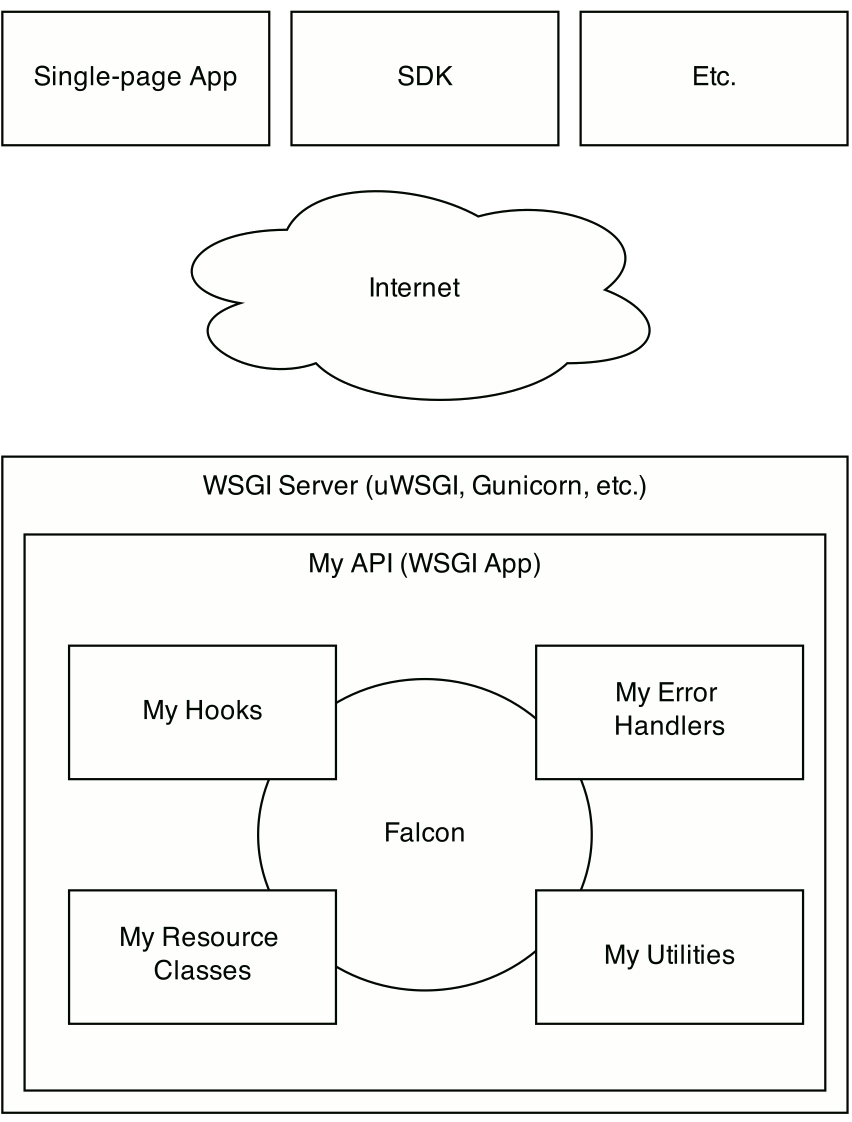
\includegraphics[width=12cm]{api_falcon.png}
% \end{center}
% \caption{Falcon Overview \cite{falcon-big-picture}}
% \label{fig:api-falcon}
% \end{figure}

